\chapter{LHC and the ATLAS detector }\label{chap:lhc}

[Thesis 2011-258]

\section{Overview}
This chapter  takes a closer look at the Large Hadron Collider located at CERN,
the European Organization for Nuclear Research, and at one of the detectors placed
along its ring: ATLAS, A Toroidal Lhc ApparatuS (described in detail in Refer-
ence [ATLAS Collaboration 2008a]).



The Large Hadron Collider (LHC) \cite{lhc1},\cite{lhc2},\cite{lhc3},\cite{lhc4} is a proton-proton collider in Geneva,
Switzerland that collides two beams of protons together at very high energies. The ATLAS
detector, which is designed to measure the output of these collisions, is located at one of
four collision points on the LHC accelerator ring. During 2012, the third year of operation,
the proton-proton collisions have been produced at a center-of-mass energy of $\sqrt{s}= 8$ TeV
with 4 TeV per proton. This center-of-mass energy has been chosen to ensure a safe
operating margin for the magnets in the accelerator, avoiding damage due to resistive
connections [85]. The design center-of-mass energy of the LHC is $\sqrt{s}= 14$.


\section{The Large Hadron Collider at CERN}
The Large Hadron Collider (LHC) is a circular accelerator located at CERN and designed
to collide beams consisting of protons or heavy-ions. It is currently the highest energy
collider in the world since it collided proton-beams at a center of mass energy of $\sqrt{s}= 7$

\subsection{Accelerator complex}

The accelerator complex at CERN is an ensemble of machines capable of accelerate particles
at increasingly higher energies. Each machine injects the beam into the next one, which takes over to bring the beam to a higher energy, and so on. The accelerator complex
is schematically shown in Figure \ref{accl}. The very first step in the chain is the proton source. The protons, extracted from Hydrogen gas, are fed into a linear accelerator (LINAC2). The LINAC2 accelerates the protons to an energy of 50 MeV. At the end of the LINAC2, the protons are injected in the Proton Synchrotron Booster (PSB), a circular accelerator in which the protons reach an energy of 1.4 GeV. At this energy, the protons are ready to be injected in a second circular accelerator,
the Proton Synchrotron (PS), in which they are accelerated up to 25 GeV. After the PS, the
protons are injected in a third circular accelerator, the Super Proton Synchrotron (SPS), in
which their energy arises to 450 GeV, which is the injection energy for the Large Hadron
Collider. The LHC is the last and more powerful step of acceleration, which boosts the proton to
4 TeV durint 2012. It is located in a circular tunnel 27 km km in circumference. The tunnel is buried about
50 to 175 meters underground. It straddles the Swiss and French borders on the outskirts
of Geneva.

\begin{figure}[h]

\includegraphics[width=\textwidth]{figs/accelerator}
\caption{
LHC accelerator complex
}
\label{accl}

\end{figure}



The beams move around the LHC ring inside a continuous vacuum guided by magnets.
The magnets are superconducting and are cooled by a cryogenics system, which makes
the LHC, not only the highest-energy collider in the world, but also the largest cryogenic
system.
The accelerator is made of eight arcs and eight "insertions". Each arc contains 154
dipole magnets. An insertion consists of a long straight section plus two (one at each end)
transition regions. The exact layout of the straight section depends on the specific use of
the insertion: physics (beam collisions within an experiment), injection, beam dumping,
beam cleaning. The important parameters that characterize the LHC with the designed
values and the values reached at the end of 2010 are listed in Table 1.1.
Once the proton bunches are injected and accelerated, the beams are stored at high
energy for hours. During this time collisions take place in the interaction points inside the
four main LHC experiments.
Figure





\subsection{Luminosity}
Besides the beam energy, the luminosity is the other characteristic that determines the
operating conditions of the LHC. The luminosity L reflects the density and rate of proton
bunches that are collided. The number of collisions per unit time, N, for a process with
a cross section $\sigma$, is determined as

\begin{equation} \label{eq:lumi1}
                N = L \times \sigma 
             \end{equation}
The luminosity is determined from the beam parameters of the accelerator:

\begin{equation} \label{eq:lumi2}
          L = \frac{N_{b}^{2} F\gamma}{4 \pi \beta^{*} \epsilon_{n}} n_{b} f_{rev}
             \end{equation}


where $N_{b}$ is the number of protons per bunch. The correction factor F arises due to
the LHC crossing angle at the interaction point, which reduces the luminous region and
prevents ``parasitic collisions'' between unintended bunches. The value of the beam envelope
function  evaluated at the interaction point,$\beta^{*}$, characterizes the beam size and
focusing distance at the collision point. The normalized transverse beam emittance, $\epsilon_{n}$,
characterizes the phase and momentum space occupied by the beam, and  is the relativistic
factor of the protons. Finally $n_{b}$ is the number of bunches and $f_{rev}$ = c/26.7 km
= 11.2 kHz is the LHC revolution frequency, where c is the speed of light.


Total Integrated Luminosity and Data Quality in 2012
The figure \ref{intlumi} shows cumulative luminosity versus time delivered to (green), recorded by ATLAS (yellow), and certified to be good quality data (blue) during stable beams and for pp collisions at 8 TeV centre-of-mass energy in 2012. The delivered luminosity accounts for the luminosity delivered from the start of stable beams until the LHC requests ATLAS to put the detector in a safe standby mode to allow a beam dump or beam studies. The recorded luminosity reflects the DAQ inefficiency, as well as the inefficiency of the so‐ called "warm start": when the stable beam flag is raised, the tracking detectors undergo a ramp of the high-voltage and, for the pixel system, turning on the preamplifiers. The data quality assessment shown corresponds to the All Good efficiency shown in the 2012 DQ table. The luminosity shown represents the preliminary 8 TeV luminosity calibration. Data quality has been assessed after reprocessing. 


\begin{figure}[H]
\begin{center}
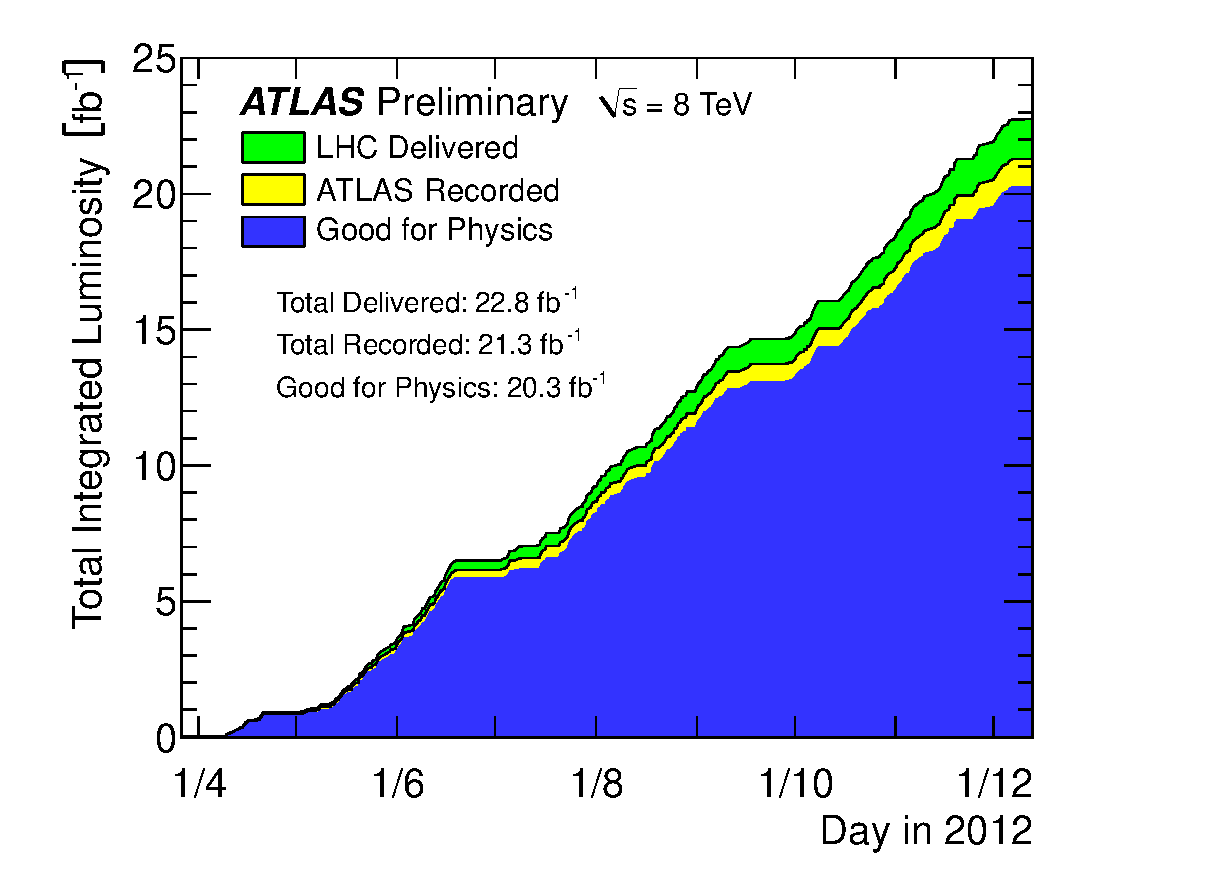
\includegraphics[width=0.8\textwidth]{figs/lumi}
\caption{
ATLAS experiment integrated luminosity for the year 2012 \cite{lumi}
}
\label{intlumi}
\end{center}
\end{figure}




\section{The ATLAS detector}
\subsection{Overview}
The ATLAS detector is a large, general-purpose particle detector that is located at Interaction
Point 1 (IP1) on the LHC accelerator ring. It is 44 m long and 25 m in diameter,
weighing about 7000 tons. It is illustrated in Fig. \ref{det} and described in detail in Ref. \cite{atlasov1}.
The overall detector has a cylindrical shape that consists of a series of many subdetectors
designed to measure the momenta of different types of particles produced in each proton-proton collision. These subdetectors are grouped into three primary systems,
which are arranged in concentric layers around the beam axis. The inner detector \cite{atlasov2},\cite{atlasov3},\cite{atlasov4},\cite{atlasov5} is a system of tracking detectors surrounded by a 2T solenoidal magnetic field. It is used for charged particle identification and position and momentum measurements. The calorimeter system \cite{atlasov6},\cite{atlasov7} is a set of calorimeters that are used to measure the energies of charged and neutral particles. The muon spectrometer \cite{atlasov8},\cite{atlasov9},\cite{atlasov10}  consists of detectors located within a large air-core toroidal magnetic field that are used to measure the position and momentum of muons.

\begin{figure}[H]
\begin{center}
\includegraphics[width=0.8\textwidth]{figs/detector}
\caption{
ATLAS detector 
}
\label{det}
\end{center}
\end{figure}


\subsection{ATLAS Coordinate system}
The ATLAS reference system is a Cartesian right-handed coordinate system, with the
nominal collision point at the origin. The counter-clockwise beam direction defines the
positive z axis, with the x axis pointing to the center of the LHC ring. The pseudorapidity
is defined as  $\eta = -ln(tan (\theta/2))$, where the polar angle, $ \theta $ , is taken with respect to the
positive z direction. The rapidity is defined as

\begin{equation} \label{eq:rapidity}
         % L = \frac{N_{b}^{2} F\gamma}{4 \pi \beta^{*} \epsilon_{n}} n_{b} f_{rev}
        y = \frac{1}{2} ln \frac{E+p_{z}}{E-p_{z}}
             \end{equation}

 where E denotes the energy and $p_{z}$ is the component of the momentum along the beam direction. In the limit of massless particles, $\eta$ = y. Since the interacting partons carry an unknown fraction of
the momenta of the colliding protons, the physical observables measured in this thesis are ratio of jet cross sections that are invariant under Lorentz boosts along the z axis.


\subsection{Inner Detector}


\subsection{Calorimeter}


\subsection{Muon Spectrometer}


\subsection{Magnet system}


\subsection{Trigger and Data acquisition}


\subsection{Detector Simulation}

%\subsection{2012 Monte Carlo samples}
%\subsection{2012 data}



